\chapter{\textit{k}-anonimity}
\label{ch.k-anon}
%Alessandro

\newtheorem{corol}{Corollario}

\newcommand{\kanon}{\textit{k}-anonimity}
\newcommand{\qi}{\textit{Quasi-Identifier}}
\newcommand{\gen}{\textit{Generalization}}
\newcommand{\supp}{\textit{Suppression}}


%%%%%%%%%%%%%%%%%%%%%%%%%%%%%%%%%%%%%%%%%%%%%%%%

Contesto è il rilascio di \textit{microdata}. 
De-identificazione non garantisce anonimità.




\section{\textit{k}-anonimity e Table \textit{k}-anonime}
Il concetto di \textit{k}-anonimity cerca di catturare sulla Private Table (PT) il vincolo che i dati rilasciati dovrebbero essere associabili in maniera indistinguibile a non meno di un certo numero di respondent.

\noindent Il set di attributi disponibili esternamente e quindi sfruttabili per fare linking è chiamato \textit{quasi-identifier}. 


\begin{definition}[\textit{k}-anonimity requirement] $\\$
    Ogni rilascio di data deve essere tale che ogni combinazione di valori del \textit{Quasi-Identifier} può essere matchata in maniera indistinguibile con almeno k \textit{respondent}.
\end{definition}


\noindent \kanon\ richiede che ogni valore del \qi abbia almeno k occorrenze nella table rilasciata, come da def  \ref{def:kanon_occorrenze} che segue:

\begin{definition}[\kanon] $\\$
    Date una table $T( A_1 , \, A_2 , \ ... A_m)$ e un insieme di attributi $QI$,  \qi\ sulla table $T$: \\
    $T$ soddisfa \kanon\ rispetto a $QI$ se e solo se ogni sequenza di valori in $T[QI]$ appare almeno con k occorrenze in $T[QI]$\footnote{ $T[QI]$ denota la proiezione con tuple duplicate degli attributi $QI$ in $T$}
\end{definition}
\label{def:kanon_occorrenze}

Definizione \ref{def:kanon_occorrenze} è sufficiente per \kanon.
Applicazione di \kanon\ richiede una preliminare identificazione del \qi.

Il \qi\ dipende dalle informazioni esterne disponibili al recipiente poichè determina le capacità di linking dello stesso.
Diversi \qi\ possono potenzialmente esistere per una data table.

Per semplicità a seguire nel paper si assume che:
\begin{itemize}
    \item PT ha unico \qi.
    \item \qi\ è composto da tutti gli attributi nella PT disponibili esternamente.
    \item PT contiene al massimo una sola tupla per ogni respondent.
\end{itemize}

\noindent \kanon\ si concentra su due tecniche di protezione: \gen\ e \supp, le quali preservano la veridicità dei dati (diversamente da swapping e scrambling).



\subsection{\gen}
Sostituzione dei valori di un attributo con valori più generali. Consideriamo:

\begin{itemize}
    \item \textit{Domain}: set di valori che un attributo può assumere.
    \item \textit{Generalized domains}: contiene valori generalizzati e relativo mapping tra ogni domain e ogni sua generalizzazione.
    \item \texttt{Dom}: set di domini originali con le loro generalizzazioni.
    \item \textit{Generalization relationship} $\leq _D$: dati $D _i , \, D _j \in $ \texttt{Dom}, $D _i \, \leq \, D_j$ significa che i valori in $D _j$ sono generalizzazioni dei valori in $D _i$. $\\$ $\\$ $\leq _D$ definisce ordinamento parziale su \texttt{Dom} ed è richiesto nelle seguenti condizioni:
\end{itemize}

\begin{condition}[C1 - Determinismo nel processo di generalizzazione] $\\$
    $\forall D_i, D_j, D_z \, $ \texttt{Dom}: $\\$
    $D_i \, \leq  _D \, D_j $, $D_i \, \leq  _D \, D_z$ $\implies$ $D_j \, \leq  _D \, D_z$ $\lor$ $D_z \, \leq  _D \, D_j$\footnote{Questo comporta che ogni dominio $D _i$ ha al massimo un solo dominio di generalizzazione diretta $D_j$ }.
\end{condition}

\begin{condition}[C2 - ] $\\$
    Tutti gli elementi massimali di \texttt{Dom} sono singoletti (singleton) \footnote{La condizione assicura che tutti i valori in ogni dominio possano essere generalizzati ad un singolo valore}.     
\end{condition}

\begin{itemize}
    \item \textbf{DGH$_D$} - \textit{Domain Generalization Hierarchy}: gerarchia di ordninamento totale per ogni dominio $D \in$ \texttt{Dom}.
\end{itemize}

\noindent Per quanto riguarda i valori nei domini consideriamo:

\begin{itemize}
    \item \textit{Value generalization relationship} $\leq _V$: associa ogni valore in $D_i$ ad un unico valore in $D_j$, sua generalizzazione.
    \item \textbf{VGH$_D$} - \textit{Value Generalization Hierarchy}: albero dove \begin{itemize}
        \item Foglie sono valori in $D$.
        \item Radice è il valore, singolo, nell'elemento massimale di DGH$_D$
    \end{itemize}
\end{itemize}



\subsection{\supp}
Consideriamo Soppressione di Tupla. "Modera" la \gen\ quando un numero limitato di \textit{outlier}\footnote{TODO outlier} forzerebbe una generalizzazione elevata.


\section{Generalizzazione \textit{k}-Minima}

\begin{definition}[Table Generalizzata con Soppressione] $\\$
    Consideriamo $T_i$ e $T_j$ due table sugli stessi attributi. $\\$
    $T_j$ è generalizzazione (con soppressione di tupla) di $T_i$, riportata come $T_i \preceq T_j$, se:
    \begin{enumerate}
        \item $|T_j| \, \leq \, |T_i|$
        \item Dominio $dom(A,T_j)$ è uguale o una generalizzazione di $dom(A,T_i)$, dove $A$ indica ogni attributo in $T_{i,j}$
        \item E' possibile definire funzione iniettiva che associa ogni tupla $t_j \in T_j$ con una tupla $t_i \in T_i$, per la quale ogni attributo in $t_j$ è uguale o generalizzazione del corrispondente in $t_i$.
    \end{enumerate}
\end{definition}

\begin{definition}[Distance Vector] $\\$
    Siano $T_i(A_1, \, ..., \, A_n)$ e $T_j(A_1, \, ..., \, A_n)$ tali che $T_i \preceq T_j$. $\\$ il distance vector di $T_j$ da $T_i$ è il vettore $\\$
    \hspace*{15pt} $DV_{i,j} \, = \, [d_1, \, ..., \, d_n]$ $\\$
    dove ogni $d_z, z=1,...,n$ è la lunghezza dell'unico percorso tra $dom(A_z,T_i)$ e $dom(A_z,T_j)$ nella $DGH_{D_z}$    
\end{definition}

\begin{corol}[Ordine Parziale tra DV] $\\$
    $DV \, = \, [d_1, \, ... , \, d_n] \, \leq \, DV' \, = \, [d'_1, \, ..., \, d'_n]$ se e solo se $d_i \, \leq d'_i$ per $i=1, \, ... , \, n$.
\end{corol}

Si costruisce una \textit{gerarchia di distance vectors} come lattice (diagramma) corrispondente alla DGH$_D$ come in fig. \ref{fig:distvect_lattice}


\begin{figure}[ht]
    \centering
    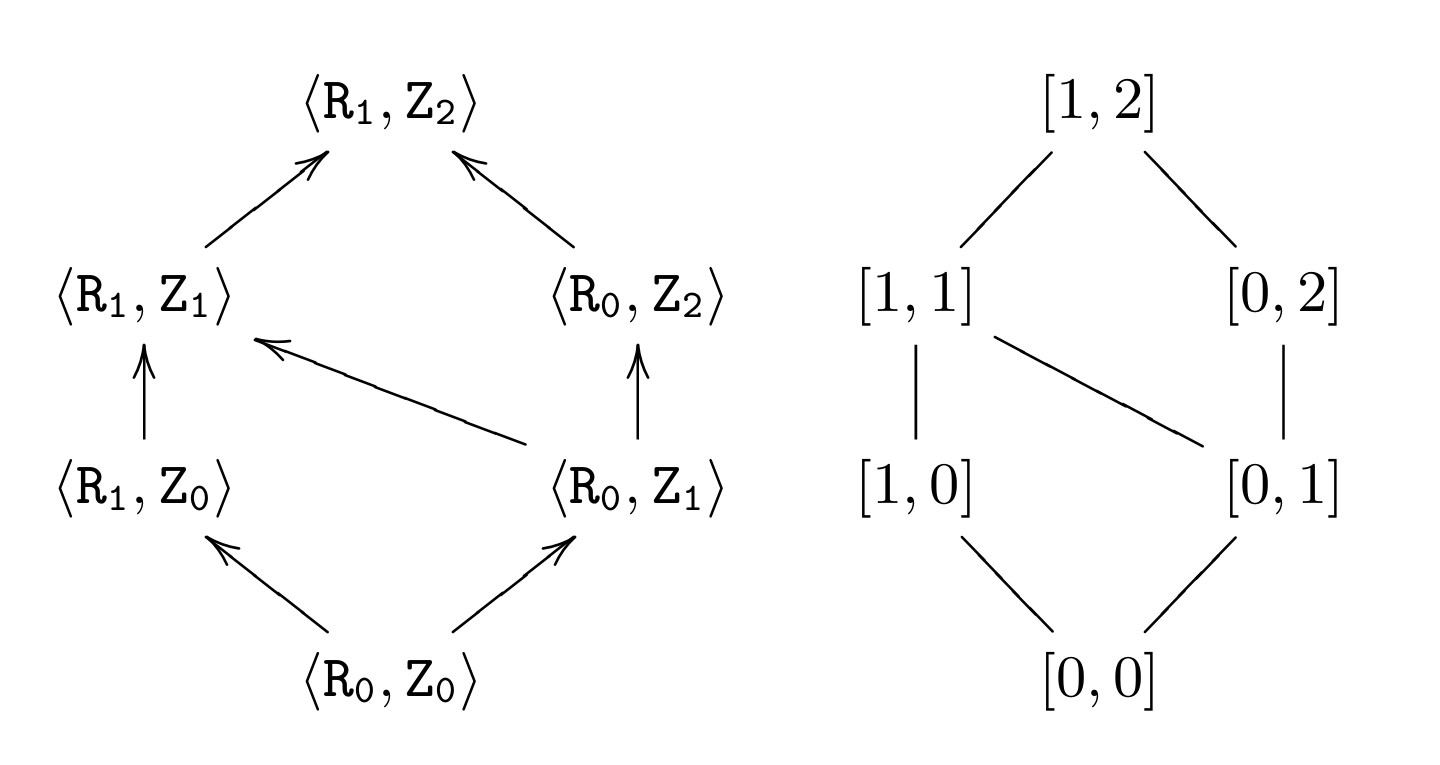
\includegraphics[width=0.5\linewidth]{paper_k-anon/DGH_e_DVgraph.jpg}
    \caption{}
    \label{fig:distvect_lattice}
\end{figure}

\newpage

Per bilanciare tra perdita di precisione dovuta a \gen\ e perdita di completezza dovuta a \supp\ si suppone che data holder determini la soglia \texttt{MaxSup}, che indica il numero di tuple che possono essere soppresse.


\begin{definition}[Generalizzazione \textit{k}-minima con Soppressione] $\\$
     Siano $T_i$ e $T_j$ due table tali che $T_i \, \preceq \, T_j$, e sia \texttt{MaxSup} la soglia di soppressione accettabile scelt. $T_j$ è una generalizzazione \textit{k}-minima di $T_i$ se e solo se: \begin{enumerate}
         \item $T_j$ soddisfa \kanon\ applicando soppressione minima, $\\$ ossia $T_j$ soddisfa \kanon\ e: $\forall T_z \, : \, T_i \preceq T_z$, $DV_{i,z} = DV_{i,j}$, $T_z$ soddisfa \kanon\ $\implies$ $|T_j| \, \geq \, |T_z|$.
         \item $|T_i| - |T_j| \, \leq $ \texttt{MaxSup}.
         \item $\forall T_z \, : \, T _i \preceq T_z$ e $T_z$ soddisfa le condizioni 1 e 2 $\implies $ $\lnot ( DV_{i,z} < DV_{i,j})$.
     \end{enumerate}    
\end{definition}

Ultima espressione rende meglio come $DV_{i,z} \geq DV_{i,j}$. Il concetto che esprime è che \textit{"non esiste un'altra \gen\ $T_z$ che soddisfi 1 e 2 con un DV minore di quello di $T_j$"} 

$\\$

\noindent Diversi \textbf{preference criteria} possono essere applicati nella scelta della generalizzazione minimale preferita:

\begin{itemize}
    \item \textbf{Distanza assoluta minima}: minor numero totale di passi di generalizzazione (indipendentemente dalle gerarchie di \gen\ considerate).
    \item \textbf{Distanza relativa minima}: minimizza il numero relativo di passi di generalizzazione (passo relativo ottenuto dividendo per l'altezza del dominio della gerarchia a cui si riferisce.
    \item \textbf{Massima distribuzione}: maggior numero di tuple distinte.
    \item \textbf{Minima soppressione}: minor tuple soppresse (maggior cardinalità).
\end{itemize}

\newpage

\section{Classificazione tecniche di \kanon}

Classificazione in fig. \ref{fig:k-anon-tech}.

\begin{figure}[ht]
    \centering
    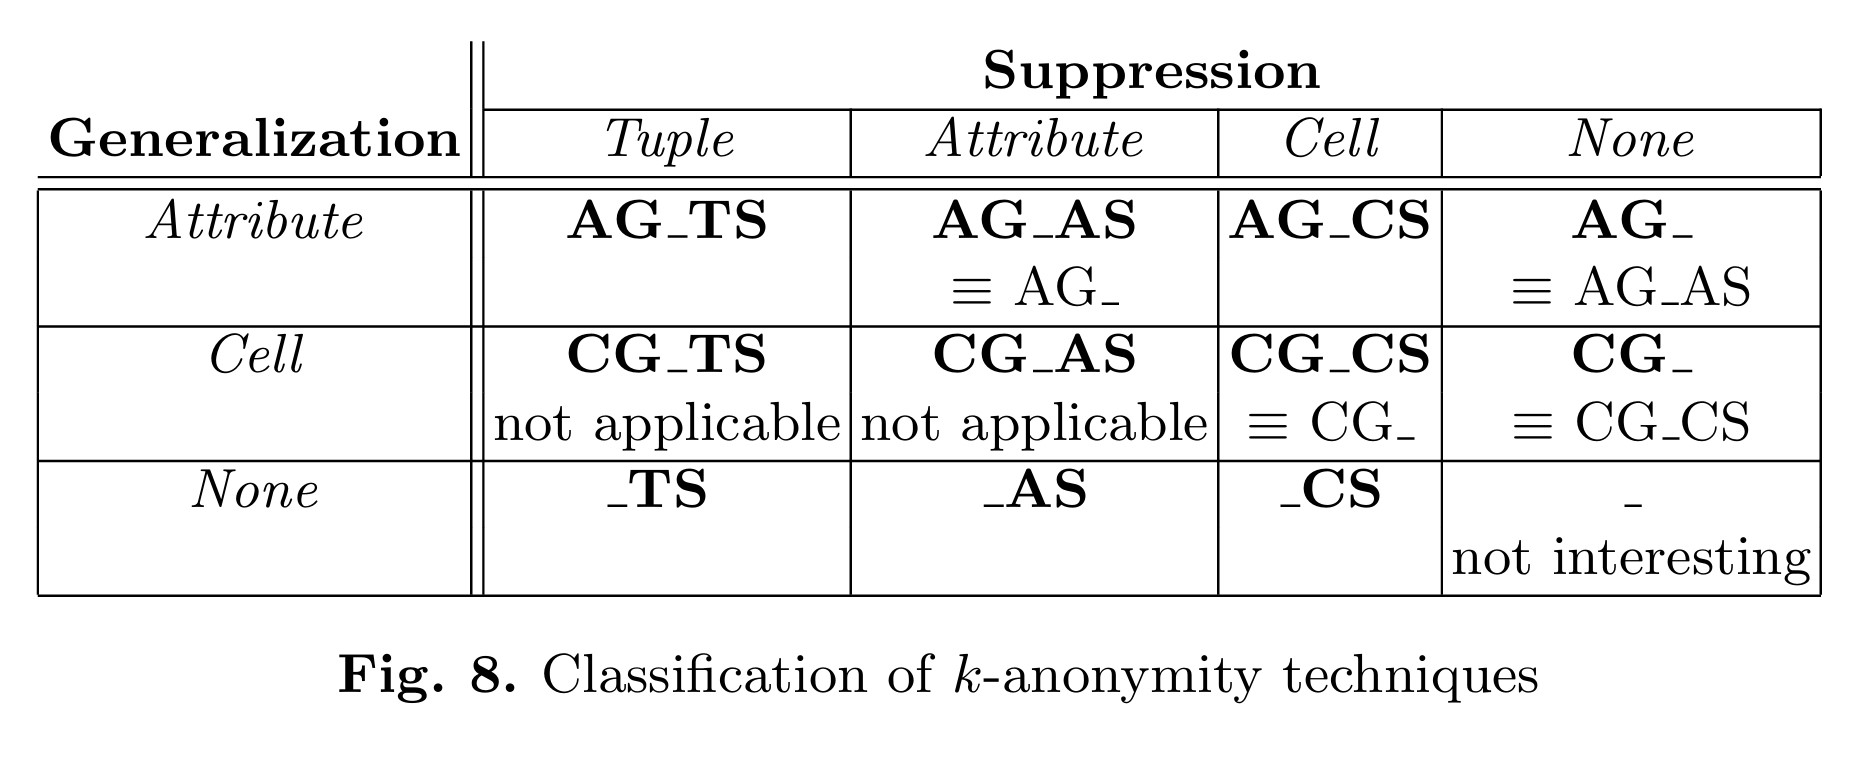
\includegraphics[width=0.8\linewidth]{paper_k-anon/k-anon-tech.jpg}
    \caption{}
    \label{fig:k-anon-tech}
\end{figure}

Casi \textit{not applicable} (\textbf{CG$\_$TS} e \textbf{CG$\_$AS}): supportare \gen\ a grana fine (cella) implica poter applicare soppressione allo stesso livello.

\begin{figure}[ht]
    \centering
    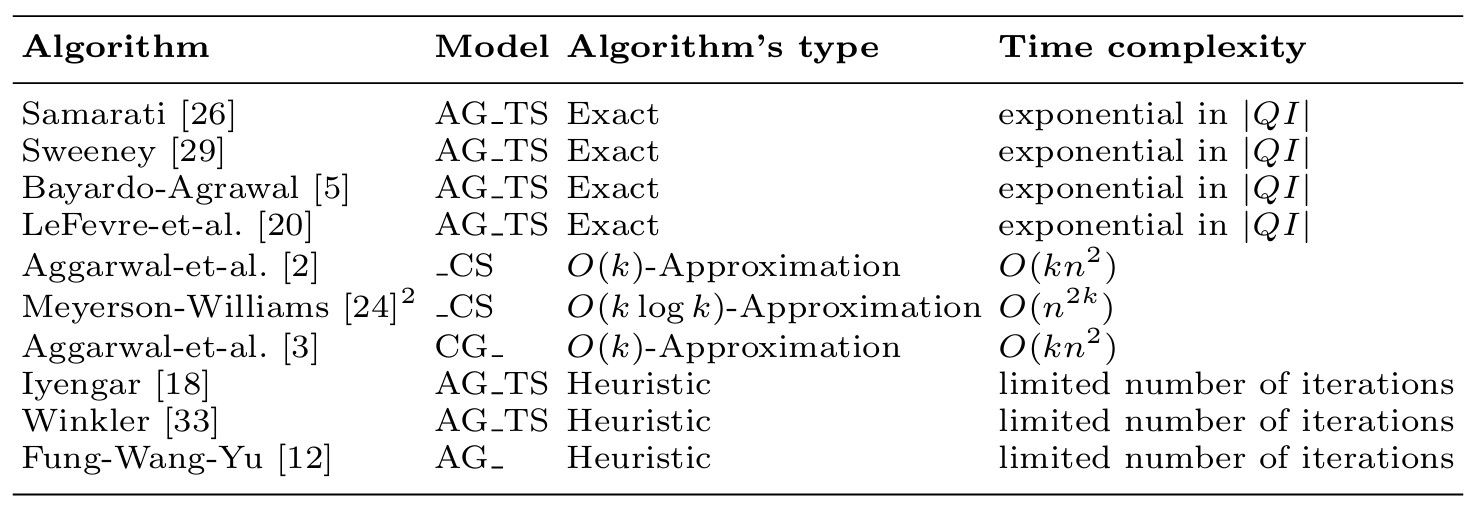
\includegraphics[width=0.8\linewidth]{paper_k-anon/k-anon-alg.jpg}
    \caption{Alcuni approcci a \kanon (\textit{n} è numero di tuple in PT).}
    \label{fig:enter-label}
\end{figure}

\section{Algoritmo Samarati (AG$\_$TS) }

Il primo algoritmo per garantire \kanon\ è stato proposto insieme alla definizione di \kanon.
La definizione di \kanon\ è basata sul QI quindi l'algoritmo lavora solo su questo set di attributi e su table con più di \textit{k} tuple. 

$\\$

\noindent Data una $DGH$ ci sono diversi percorsi dall'elemento in fondo alla gerarchia alla radice. Ogni percorso è una differente \textit{strategia} di generalizzazione.
Su ogni percorso c'è esattamente una \gen\ minima localmente (nodo più basso che garantisce \kanon).

\noindent In maniera naif si può cercare su ogni percorso il minimo locale per poi trovare il minimo globale tra questi ma non è praticabile per l'elevato numero di percorsi.

$\\$

\noindent Per ottimizzare la ricerca si sfrutta la proprietà che salendo nella gerarchia la soppressione richiesta per avere \kanon\ diminuisce:

\begin{itemize}
    \item Ogni nodo in $DGH$ viene associato ad un numero, \textbf{height}, corrispondente alla somma degli elementi nel Distance Vector associato.
    \item Altezza di ogni DV nel diagramma (\textit{distance vector lattice} \texttt{VL}) si scrive come \textit{height}($DV$,\texttt{VL}).
\end{itemize}

Se non c'è soluzione che soddisfi \kanon\ sopprimendo meno di \texttt{MaxSup} ad altezza \textit{h} non può esistere soluzione che soddisfi ad una altezza minore.


$\\$

\noindent L'algoritmo usa binary search cercando la minore altezza in cui esiste un $DV$ che soddisfa \kanon\ rispettando \texttt{MaxSup} e ha come primo passo:

\begin{equation}
    \text{Cerco ad altezza } \lfloor \frac{h}{2} \rfloor : \begin{cases}
        \text{trovo vettore che soddisfa \kanon} \, \implies \lfloor \frac{h}{4} \rfloor \\
        \text{altrimenti } \implies \text{cerco in} \, \lfloor \frac{3h}{4} \rfloor
    \end{cases}
\end{equation}

\noindent La ricerca prosegue fino a trovare l'altezza minore in cui esiste vettore che soddisfa \kanon\ con \texttt{MaxSup}.

\subsection{Evitare il calcolo delle table generalizzate}

\noindent Algoritmo richiederebbe il calcolo di tutte le table generalizzate.
Per evitarlo introduciamo il concetto di $DV$ tra tuple.

\begin{definition}[Distance Vector tra tuple - Antenato Comune] $\\$
    Sia $T$ una table. $\\$ 
    Siano $x,y \in T$ due tuple tali che $x = \langle v'_1 , \, ..., \, v'_n \rangle$ e $y = \langle v''_1 , \, ..., \, v''_n \rangle$ con $v'_i$ e $v''_i$ valori in $D_i$ con $i=1, \, ..., \, n$. $\\$
    Il \textbf{distance vector} tra $x$ e $y$ è $V_{x,y}= [d_1, \, ..., \, d_n]$. dove $d_i$ è la lunghezza (uguale) dei due percorsi da $v'_i$ e $v''_i$ al loro comune antenato comune più prossimo $v_i$ sulla $VGH_{D_i}$. 
\end{definition}

$\\$

\noindent In altri termini ogni distanza in $V_{x,y}$ è una distanza uguale dal dominio di $v'_i$ e $v''_i$ al dominio in cui sono generalizzati allo stesso valore $v_i$.

\noindent Allo stesso modo $V_{x,y}$ per $x,y \in T_i$ equivale a $DV_{i,j}$ per $T_i \preceq T_j$ per cui $x$ e $y$ vengono generalizzate alla stessa tupla $t$.

$\\$

\textbf{Per il momento il resto è delirio}





\newpage

\section{Bayardo-Agrawal: \textit{k-Optimize} (AG$\_$TS) }

Approccio considera che la generalizzazione di attributo $A$ su dominio \textbf{ordinato} $D$ corrisponde ad un partizionamento del dominio dell'attributo in intervalli.  
Ogni valore del dominio deve comparire in un intervallo e ogni valore in un intervallo precede ogni valore degli intervalli che lo seguono.

Si assume quindi un ordine tra gli attributi del \qi. Inoltre associa un valore intero chiamato \textit{index} ad ogni intervallo di ogni dominio degli attributi del \qi.


$\\$
Una \gen\ è quindi rappresentata come l'unione dei valori di indice per ogni attributo (il valore più piccolo in un dominio viene omesso perchè comparirà sicuramente nella generalizzazione per quel dominio).

\textit{k-Optimize} costruisce un \textit{set enumeration tree} sul set $I$ di valori di indice, con radice vuota.
Ogni nodo figlio è costruito dal padre inserendo in coda un index di $I$ maggiore degli altri index già presenti nel padre (per ordinamento totale).


$\\$
La visita dell'albero permette di valutare con Depth First Search ogni nodo, prunando ogni nodo e tutti i suoi figli se questi non possono corrispondere a soluzioni ottimali.
Nello specifico \textit{k-Optimize} pruna un nodo $n$ quando determina che nessuno dei suoi discendenti può essere ottimale. Data una funzione di costo l'algoritmo calcola un limite inferiore sul costo che può essere ottenuto sul subtree del nodo $n$, prunando se nodo a costo minore è già stato trovato.

$\\$
Se un nodo viene prunato allora anche altri nodi, non per forza del sottoalbero, possono essere prunati: supponendo di prunare il nodo $\{$1,3$\}$ in figura \ref{fig:set_enum_tree} allora posso prunare qualunque altro nodo contenente $1$ E $3$, come ad esempio $\{$1,2,3$\}$.

\begin{figure}[h]
    \centering
    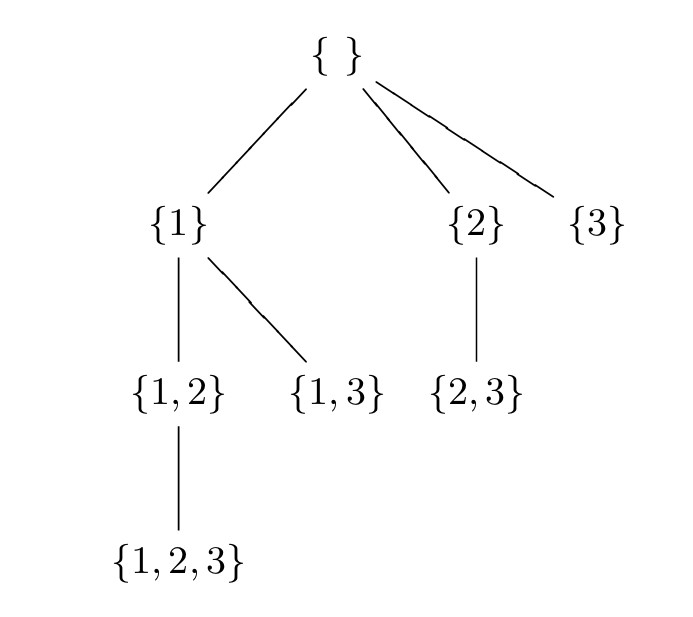
\includegraphics[width=0.4\linewidth]{paper_k-anon/set_enum_tree}
    \caption{Set enumeration tree sull'insieme di indici I=$\{$1,2,3$\}$}
    \label{fig:set_enum_tree}
\end{figure}





\section{LeFevre-DeWitt et al.: Incognito (AG$\_$TS) }

Aggregazione bottom-up.

$\\$
Idea di base è riassunta nella seguente definizione:

\begin{definition} $\\$
    Se una table $T$ con \qi\ $QI$ composto da $m \, = |QI|$ attributi soddisfa \kanon, $T$ soddisfa \kanon\ anch per qualunque \qi\ $QI'$ talce che $QI' \subset QI$.
    
    Pertanto \kanon\ su un subset di $QI$ è condizione necessaria (e non sufficiente) per \kanon\ di $T$ sull'intero $QI$.
\end{definition}


Algoritmo esclude in anticipo alcune generalizzazioni della gerarchia con un calcolo a priori.

$\\$
Strategia: bottom-up BFS sulla $DGH$. 
Incognito genera tutte le possibili table \textit{k}-anonime minime secondo i seguenti passaggi:

\begin{enumerate}
    \item (Iterazione 1): verifica \kanon\ per ogni singolo attributo nel \qi, scartando quelle che non soddisfano.
    \item (Iterazione 2): combina a coppie le \gen\ non scartate al passo 1 verificando \kanon.
    \item (...)
    \item (Iterazione $m$): arriva a considerare l'intero set di attributi di $QI$  
\end{enumerate}

\noindent Utilizzando approccio bottom-up, per la condizione citata prima, se una \gen\ soddisfa \kanon\ allora anche sue ulteriori dirette generalizzazioni soddisfano \kanon\ e pertanto non sono considerate ulteriormente.

